\documentclass[11pt,letterpaper]{article}

% ---------- packages ----------
\usepackage{iftex}
\ifXeTeX
  \usepackage{fontspec}          % Latin Modern by default
\else
  \usepackage[T1]{fontenc}
  \usepackage[utf8]{inputenc}
  \usepackage{lmodern}
\fi
\usepackage[margin=1in]{geometry}
\usepackage{graphicx}
\usepackage{booktabs,tabularx,xltabular,array}
\usepackage{enumitem}
\usepackage[font=small,labelfont=bf]{caption}
\usepackage{float}
\usepackage{amssymb}
\usepackage{textcomp}
\usepackage{xcolor}
\usepackage{tikz}
\usetikzlibrary{positioning,fit,shapes.geometric,arrows.meta,calc}
\usepackage[hyphens]{url}
\usepackage[hidelinks]{hyperref}
\usepackage{microtype}
\usepackage{needspace}

\setlist{itemsep=2pt,topsep=3pt}
\setlength{\parindent}{0pt}
\setlength{\parskip}{4pt}
\renewcommand{\arraystretch}{1.2}
\urlstyle{tt}

\newcommand{\code}[1]{\path{#1}}
\newcommand{\prompt}[1]{\par\needspace{10\baselineskip}\medskip{\itshape #1}\par\smallskip}
\newcommand{\lead}[1]{\textbf{#1}~}
\newcolumntype{L}[1]{>{\raggedright\arraybackslash}p{#1}}
\newcolumntype{Y}{>{\raggedright\arraybackslash}X}
\newcolumntype{C}{>{\centering\arraybackslash}X}

\title{Fair Visibility for Local News on Google News Canada\\[4pt]
\large INSE 6450: AI in Systems Engineering, Milestone 2\\[2pt]
\normalsize Model Selection, Training, Efficiency, and Deployment}
\author{
Maria Camila Guzman \\ \small 40239038 \and
David Esuga-Mopah \\ \small 40368321 \and
Ege Karadibak \\ \small 40080456 \and
J. David Ruiz \\ \small 40176885}
\date{Concordia University, Fall 2026 \\ October 26, 2026}

\begin{document}
\maketitle


% =====================================================================
\section{Model Selection}

\subsection{Plausible Model Families}

Our model decides whether two headlines describe the same news story. It is trained on pairs built from Google News Canada's Top Stories cards. Two headlines in the same card form a positive pair (same story), and two headlines from different cards in the same snapshot form a negative pair (different story). The model's similarity scores are then used to group articles into story cards.

{\small
\begin{xltabular}{\linewidth}{L{3.3cm}YY}
\caption{Candidate model families.}\\
\toprule
\textbf{Model family} & \textbf{Why it fits our data and objective} & \textbf{Why it might not be ideal} \\
\midrule
\endhead

Linear model on lexical features (TF-IDF vectors with cosine similarity)
& The simplest way to compare headlines. It is fast, runs on a CPU and is easy to interpret, since you can see which shared words drive a match. It serves as our lexical baseline to check whether a neural model is needed.
& It only matches exact words, so the same event described in different words looks unrelated, and English and French headlines cannot be compared at all. It also cannot tell that common names such as ``Carney'' or ``Trump'' appear across many different stories. \\
\midrule
Transformer bi-encoder (paraphrase-multilingual-MiniLM-L12-v2, pretrained or fine-tuned on our same-story/different-story pairs)
& It is trained for paraphrase similarity, so it recognizes the same story told in different words. It maps English and French headlines into one vector space. Each headline is embedded once and then compared with others using cheap vector operations, which suits clustering and a browser extension. Fine-tuning adapts it to Google's notion of ``same story'' using labels we already have.
& The model is 471\,MB on disk, which is heavy relative to our dataset, and it is slower than TF-IDF. Fine-tuning on 21,907 training pairs can overfit, so it needs a time-based validation split and early stopping. It is less interpretable than a linear model. \\
\midrule
Transformer cross-encoder (both headlines fed together into one multilingual transformer that outputs a same-story probability)
& It reads both headlines at once and compares them word by word, which is usually more accurate than comparing two separate vectors, especially for close calls such as two different stories about the same politician.
& It must run the transformer once for every pair of headlines instead of once per headline, so scores cannot be precomputed and reused. We trained one for comparison (Section~\ref{sec:training}): it matched the bi-encoder's test F1 (0.906) and grouped cards slightly better, but it was about 7.5 times slower per page (122\,ms vs.\ 16\,ms on a laptop CPU, Section~\ref{sec:efficiency}). \\
\bottomrule
\end{xltabular}}

\subsection{Selected Model and Justification}

We selected a fine-tuned multilingual transformer bi-encoder (paraphrase-multilingual-MiniLM-L12-v2). It is trained on headline pairs from Google's cards to recognize when two headlines describe the same story. TF-IDF and the pretrained MiniLM, without fine-tuning, serve as baselines that the fine-tuned model must beat (Table~\ref{tab:baselines}).

\begin{table}[H]
\centering\small
\resizebox{\linewidth}{!}{%
\begin{tabular}{llrrrrrrrrr}
\toprule
Baseline & Split & Threshold & Precision & Recall & F1 & Accuracy & ROC-AUC & PR-AUC & Pairs & Seconds \\
\midrule
TF-IDF & val  & 0.042 & 0.862 & 0.739 & 0.795 & 0.828 & 0.862 & 0.873 & 2,850 & 0.054 \\
TF-IDF & test & 0.042 & 0.868 & 0.688 & 0.768 & 0.805 & 0.834 & 0.846 & 2,457 & 0.046 \\
MiniLM pretrained & val  & 0.294 & 0.810 & 0.857 & 0.833 & 0.844 & 0.923 & 0.911 & 2,850 & 2.443 \\
MiniLM pretrained & test & 0.294 & 0.893 & 0.836 & 0.863 & 0.876 & 0.947 & 0.945 & 2,457 & 0.428 \\
\bottomrule
\end{tabular}}
\caption{Baselines on the validation and test pairs. The threshold is chosen on validation and applied unchanged to test.}
\label{tab:baselines}
\end{table}

\prompt{Match to task type: classification, regression, forecasting, anomaly detection, retrieval, etc.}

The core task is pairwise binary classification: given two headlines, predict ``same story'' or ``different story.'' The bi-encoder outputs a cosine similarity, and a threshold turns that score into a decision. We choose the threshold on the validation set as the value with the highest F1 and apply it unchanged to the test set. We evaluate with precision, recall and F1 against Google's cards. The same similarity scores then feed a clustering step that groups articles into story cards.

\prompt{How the model's inductive biases fit your features from Phase 1.}

\begin{itemize}
\item \lead{Meaning over wording:} The model assumes that headlines with similar meaning should have nearby vectors even when they share few words. Our baselines confirm that this matters. TF-IDF reached high precision (0.868) but low recall (0.688) on the test set, and its best threshold was only 0.042, showing that many same-story headlines share almost no words. The pretrained MiniLM reached a recall of 0.836.
\item \lead{Shared bilingual space:} In Phase 1 we planned multilingual embeddings because headlines are in English and French. The model maps both languages into one space: in a quick check, an English and a French headline about the same event scored 0.736, while an unrelated pair scored $-0.053$.
\item \lead{Learning from existing labels:} Fine-tuning pulls same-card headlines together and pushes different-card headlines apart. The model learns Google's notion of a story from 21,907 labelled training pairs with no manual labelling.
\item \lead{Text only:} Consistent with Phase 1, the model sees only headline text, never publisher identity. Timing enters as a constraint rather than a feature: pairs and clusters are formed within the same snapshot, so articles from different time periods are never compared.
\end{itemize}

\prompt{Expected accuracy and robustness versus complexity, latency, and memory.}

\begin{itemize}
\item \lead{Accuracy:} The pretrained MiniLM already outperforms TF-IDF on test (F1 0.863 vs.\ 0.768; ROC-AUC 0.947 vs.\ 0.834). This makes it a strong starting point, so we expected fine-tuning to bring smaller gains on top of it. The fine-tuned model had to exceed test F1 0.863 and ROC-AUC 0.947 to be adopted; it reached 0.906 and 0.971 (Section~\ref{sec:training}). A fine-tuned cross-encoder matched its test F1 but was 7.5 times slower per page and cannot reuse precomputed scores, so the bi-encoder is the deployed model.
\item \lead{Robustness:} We train on articles before 2026, validate on January--April 2026 and test from May 2026 onward, so the model is always evaluated on news it has not seen. Validation and test results are consistent (pretrained MiniLM F1 0.833 on validation, 0.863 on test). The pairs are nearly balanced (47.6\%, 45.3\% and 46.8\% same-story pairs in train, validation and test), so no re-weighting or resampling is needed. Early stopping on validation PR-AUC limits overfitting to the training pairs.
\item \lead{Cost:} Fine-tuning keeps the same architecture (471\,MB pretrained, 488\,MB fine-tuned on disk), so it adds no inference cost. The pretrained model scored the 2,457 test pairs in 0.43\,s on our laptop, while TF-IDF took 0.05\,s.
\end{itemize}

\subsection{Architecture Details}

\prompt{Input representations and preprocessing.}

\begin{itemize}
\item \lead{Source:} Top Stories articles (``Top stories'' and ``\`A la une'') from \code{front_page_articles.csv}, main snapshots only (same-day repeat snapshots and the 5 snapshots the Archive served from the wrong date removed).
\item \lead{Cards:} grouped by timestamp, edition and card number, not \code{story_id}, which is empty for about half the rows. Only cards with 2 or more articles are kept. This leaves 2,178 cards (2,112 with 4 articles and 66 with 3) from 1,267 snapshots, totalling 8,646 articles. Our article counts match Google's \code{cluster_size} for every card.
\item \lead{Pairs:} two headlines in the same card are labelled 1, and two headlines from different cards in the same snapshot are labelled 0. This gives 27,230 raw pairs.
\item \lead{Cleaning:} we drop pairs with identical text and pairs that receive both labels, keep each pair once per split, and remove validation and test pairs already seen in an earlier split to prevent leakage. 27,214 pairs remain.
\item \lead{Text:} headlines are Unicode-normalized (NFC) and whitespace is collapsed. Inputs are truncated at 128 tokens, and MiniLM outputs 384-dimensional L2-normalized embeddings, so cosine similarity is a dot product.
\item \lead{Temporal split:} see Table~\ref{tab:split}.
\end{itemize}

\begin{table}[H]
\centering\small
\begin{tabular}{llrrr}
\toprule
Split & Period & Same story (1) & Different story (0) & Total \\
\midrule
Train      & before Jan 2026 & 10,420 & 11,487 & 21,907 \\
Validation & Jan--Apr 2026   & 1,290  & 1,560  & 2,850 \\
Test       & May 2026 onward & 1,149  & 1,308  & 2,457 \\
\bottomrule
\end{tabular}
\caption{Temporal split of the labelled headline pairs.}
\label{tab:split}
\end{table}

\prompt{Main architecture and hyperparameters (e.g., depth, width, embeddings, loss, regularization, early stopping, augmentation).}

{\small
\begin{xltabular}{\linewidth}{L{3.6cm}Y}
\toprule
Component & Setting \\
\midrule
\endhead

Encoder & paraphrase-multilingual-MiniLM-L12-v2: 12 transformer layers, hidden size 384, 118M parameters (471\,MB pretrained, 488\,MB fine-tuned) \\
Output & 384-dimensional L2-normalized embedding per headline; pair score = cosine similarity \\
Decision rule & score $\geq$ threshold $\rightarrow$ same story; threshold chosen on validation as the value with the highest F1: 0.724 for the fine-tuned model (0.294 pretrained) \\
Fine-tuning loss & Online contrastive loss on cosine distance (margin 0.5). In each batch it pulls together same-story pairs that are still far apart and pushes apart different-story pairs that are still too close. \\
Regularization & Word-embedding table frozen (96M of 118M parameters; 21.6M trained); AdamW weight decay 0.01; gradient clipping at 1.0; early stopping on validation PR-AUC (patience 1) \\
Augmentation & None in the final model. We tested four (boilerplate stripping, hard negatives, mined positives, English$\leftrightarrow$French translation); none improved validation F1 (Section~\ref{sec:results}). \\
Grouping into cards & Within each page: agglomerative clustering (average linkage) on cosine distance, cut at 1 $-$ threshold. Headlines join a card when they are on average more similar than 0.724. \\
TF-IDF baseline & Word unigrams and bigrams, lowercased, accents stripped, sublinear term frequency, fitted on training headlines only \\
\bottomrule
\caption{Architecture and hyperparameters of the selected model.}
\end{xltabular}}

\prompt{Versioned configuration (e.g., seed, learning rate, batch size, optimizer).}

{\small
\begin{xltabular}{\linewidth}{L{3.6cm}Y}
\toprule
Setting & Value \\
\midrule
\endhead

Seed & 6450 (same as Phase 1 sampling) \\
Optimizer & AdamW (weight decay 0.01), linear warm-up over the first 10\% of steps, then linear decay \\
Learning rate & $2 \times 10^{-5}$ \\
Batch size & 32 pairs for fine-tuning; 64 headlines for embedding \\
Epochs & At most 3, early stopping on validation PR-AUC (patience 1). Best epoch: 1 (stopped after epoch 2) \\
Model storage & \code{models/} (gitignored); shared with the team on Google Drive \\
Code & \code{src/build_pairs.py}, \code{src/embeddings.py}, \code{src/baselines.py}, \code{src/m2_common.py}; \code{milestone2_training.ipynb}, \code{milestone2_experiments.ipynb}, \code{milestone2_label_noise.ipynb}. Libraries are listed in \code{requirements.txt}; exact versions and hardware are saved with each run in \code{outputs/milestone2/train_config.json} \\
\bottomrule
\caption{Versioned training configuration.}
\end{xltabular}}


% =====================================================================
\section{Training and Experimentation}
\label{sec:training}

\subsection{Training Procedure}

\lead{Train/validation/test methodology.} The split is temporal, not random: train uses pages before 2026 (21,907 pairs), validation January--April 2026 (2,850), and test May 2026 onward (2,457). The model is therefore always evaluated on later news it has never seen, and pairs that already appear in an earlier split are removed. No stratification was needed, since every split is 45--48\% same-story pairs. The test set is 75\% English, so we also report results per language.

\lead{Hyperparameter tuning.} Manual. The optimizer settings (Section~1.3) are standard for fine-tuning sentence-transformer models and were not searched. The decision threshold is tuned on validation (best F1) and applied unchanged to test. What we varied, one change at a time and judged on validation only, was the training data (four augmentations) and the architecture (bi-encoder vs.\ cross-encoder). The test set was used once, at the end.

\lead{Hardware, epochs and early stopping.} NVIDIA RTX 3080 (10\,GB VRAM), 16-thread Intel CPU, 34\,GB RAM; Python 3.12, PyTorch 2.9 (CUDA 12.8), sentence-transformers 6.2. Training runs for at most 3 epochs, with early stopping on validation PR-AUC (patience 1). The best epoch was epoch 1, and training stopped after epoch 2 (0.7\,min per epoch, 1.5\,min total).

\needspace{0.45\textheight}
\subsection{Experimental Results}
\label{sec:results}

\prompt{Learning curves: loss and relevant metric versus epochs or steps.}

\begin{figure}[H]
\centering
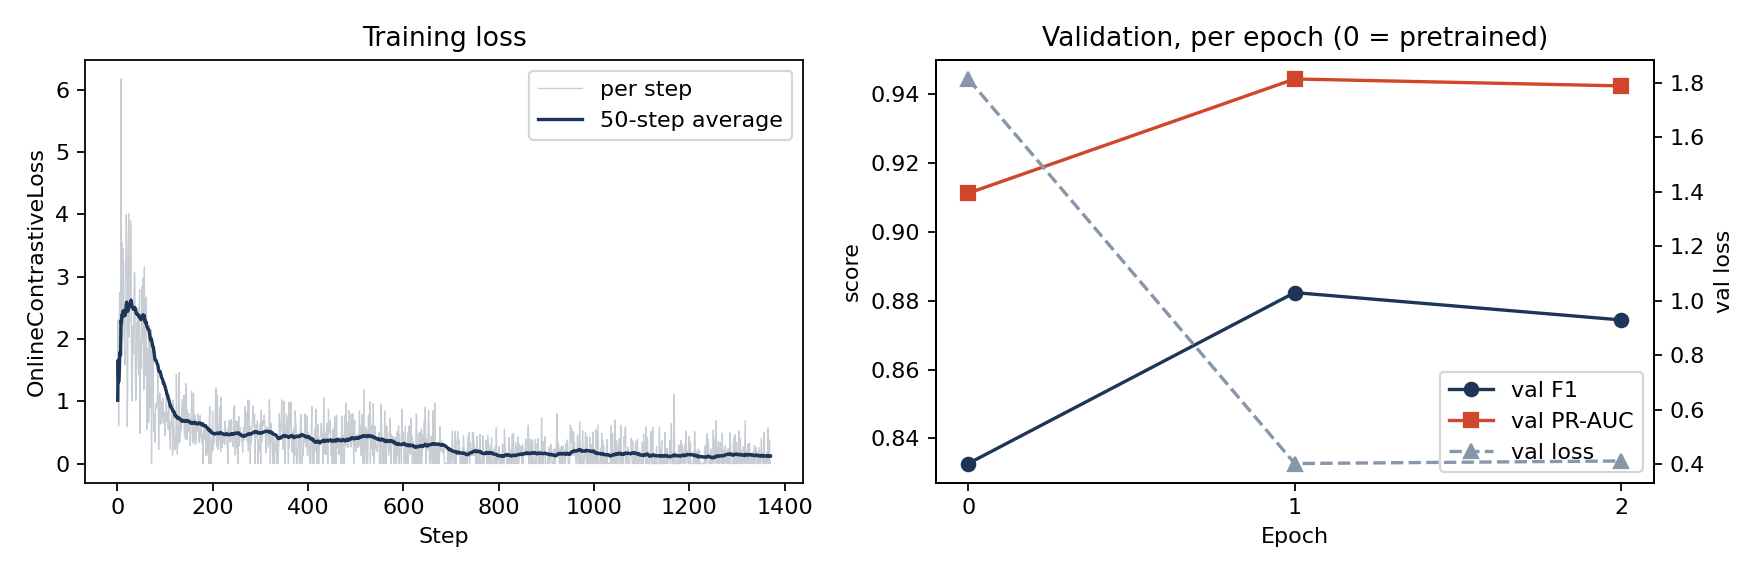
\includegraphics[width=\linewidth]{figures/learning_curves.png}
\caption{Left: training loss per step. Right: validation F1, PR-AUC and loss per epoch (epoch 0 is the pretrained model).}
\end{figure}

Training loss falls from 2.31 to 0.12 (average of the first vs.\ last 50 steps). Validation F1 rises from 0.833 (pretrained, epoch 0) to 0.882 after epoch 1, then drops to 0.874 after epoch 2 while validation loss rises slightly (0.403 $\rightarrow$ 0.413). The model starts to overfit after one epoch, so early stopping keeps epoch 1.

\prompt{At least one ablation or comparison (e.g., baseline versus final model, smaller versus larger model, key feature enabled versus disabled).}

\begin{table}[H]
\centering\small
\begin{tabular}{lrrrrr}
\toprule
Model & F1 & ROC-AUC & PR-AUC & Card ARI & Exact cards \\
\midrule
TF-IDF & 0.768 & 0.834 & 0.846 & 0.640 & 58\% \\
Pretrained MiniLM & 0.863 & 0.947 & 0.945 & 0.702 & 60\% \\
\textbf{Fine-tuned bi-encoder (deployed)} & \textbf{0.906} & \textbf{0.971} & \textbf{0.966} & 0.776 & 67\% \\
Fine-tuned cross-encoder & 0.906 & 0.970 & 0.964 & 0.814 & 71\% \\
\bottomrule
\end{tabular}
\caption{Ablation 1: baselines vs.\ final model on the test set.}
\end{table}

Fine-tuning removes about a third of the pretrained model's errors. The cross-encoder matches the pair F1 and groups pages into cards slightly better, but it is 7.5 times slower per page (Section~\ref{sec:efficiency}), so we deploy the bi-encoder. Card ARI measures agreement with Google's cards (1 means identical); exact cards is the share of Google's cards reproduced exactly.

\begin{table}[H]
\centering\small
\begin{tabular}{lrrr}
\toprule
Training data & All & English & French \\
\midrule
None (pretrained) & 0.863 & 0.862 & 0.866 \\
English pairs only & 0.886 & 0.895 & 0.858 \\
\textbf{English and French pairs} & \textbf{0.906} & \textbf{0.917} & \textbf{0.875} \\
\bottomrule
\end{tabular}
\caption{Ablation 2: training languages (test F1).}
\end{table}

Training on English only makes French worse than no training at all. Training on both languages is what carries the gain over to French.

\lead{Other changes tried} (validation F1; v1 = 0.882): boilerplate stripping 0.881, hard negatives 0.872, mined positives 0.878, English$\leftrightarrow$French translation 0.879. None improved on the model without them, so the final model uses none. The reasons:
\begin{itemize}
\item \lead{Too small to matter:} two of the changes touched very little data (177 headlines; 136 pairs).
\item \lead{Wrong skill:} translation teaches cross-language matching, which the same-language validation set does not measure.
\item \lead{Fuzzy labels:} ``different story'' is unclear across days, so the hard negatives added wrong labels.
\end{itemize}

\lead{Class imbalance.} None: every split is 45--48\% same-story pairs, so no re-weighting, focal loss or resampling was used.

\subsection{Task Metrics}

The model classifies headline pairs and groups them into cards. The order of articles inside a card is set by a fixed rule, not learned. So we report classification metrics (precision, recall and F1 at the validation threshold, plus threshold-free ROC-AUC and PR-AUC) and card-level clustering metrics, rather than NDCG@K.

\begin{table}[H]
\centering\small
\begin{tabular}{lrrrrrr}
\toprule
Fine-tuned bi-encoder & Precision & Recall & F1 & Accuracy & ROC-AUC & PR-AUC \\
\midrule
Validation (2,850 pairs) & 0.884 & 0.881 & 0.882 & 0.894 & 0.950 & 0.944 \\
Test (2,457 pairs)       & 0.916 & 0.896 & 0.906 & 0.913 & 0.971 & 0.966 \\
\bottomrule
\end{tabular}
\caption{Task metrics of the deployed model.}
\end{table}

F1 by language is 0.901 English / 0.863 French on validation, and 0.917 / 0.875 on test. On test pages the model groups articles into cards with an ARI of 0.776 against Google's cards.

Our labels come from Google's cards, which are sometimes wrong themselves. In a hand check of 150 validation pairs that the models disputed (a first pass by an AI assistant), Google's label was wrong in 8\% and unclear in 30\%. Against corrected labels, leaving out the unclear pairs, the estimated validation F1 is 0.932 (95\% interval 0.914--0.948).


% =====================================================================
\section{Efficiency Metrics: Training and Inference}
\label{sec:efficiency}

The model we deploy is the fine-tuned MiniLM bi-encoder. It turns each headline into a vector, and if two vectors are close enough we treat the headlines as the same story. Because each headline gets its own vector, we can embed headlines once when they are published and store them, so a user's request mostly just compares vectors that are already saved. We also measured the cross-encoder from our experiments. It has to read both headlines together, so nothing can be computed ahead of time, and we mainly include it to show why we did not pick it.

\subsection{Training Efficiency}

We trained on an NVIDIA RTX 3080 with a batch size of 32.

\begin{itemize}
\item \lead{Total training time:} 1.5\,min across two epochs. Early stopping was triggered after the second epoch, so we retained the model from epoch 1.
\item \lead{Time per epoch:} 0.7\,min.
\item \lead{Steps per second:} 16.68.
\item \lead{Peak memory:} 2.63\,GB of RAM and 1.83\,GB of VRAM.
\item \lead{Model size:} 117.65 million parameters in total, of which 21.6 million are trainable. We froze the word-embedding table, which contains approximately 96 million parameters. The saved model occupies 487.7\,MB on disk.
\item \lead{FLOPs:} We measured floating-point operations using PyTorch's \texttt{FlopCounterMode} on real training batches. Each training pair requires approximately 3.0 GFLOPs, including the forward and backward passes. Across the full run (21,907 pairs $\times$ 2 epochs), the training steps require approximately $1.3 \times 10^{5}$ GFLOPs, plus a small additional amount for validation scoring. At inference, each pair requires approximately 2.1 GFLOPs.
\item \lead{Energy and cost:} We did not measure power consumption. Assuming the GPU continuously drew its full rated 320\,W, 1.5 minutes of training would consume approximately 8\,Wh of GPU energy. This excludes the rest of the system, and the electricity cost depends on the local rate. With our existing hardware, the short training time makes retraining practical whenever more labelled data becomes available.
\end{itemize}

\subsection{Inference Efficiency}

\prompt{Measure the following on your available hardware, specifying the CPU/GPU and batch size.}

We measured inference on an Apple M4 Max laptop using only the CPU, with 10 threads, PyTorch 2.8 and fp32 precision. This evaluates CPU deployment, although performance on other laptops and server hardware may differ. We tested three workloads, and every timing includes tokenization:

\begin{itemize}
\item \lead{Single pair:} batch size 1, used to measure latency for one pair of headlines.
\item \lead{Batch processing:} batch size 64, used to measure batch latency and throughput.
\item \lead{Page processing:} a representative Google News front page containing nine headlines, giving 36 unique headline pairs.
\end{itemize}

\paragraph{Latency and throughput.}
\begin{itemize}
\item \lead{Single-pair latency:} 7.6\,ms at p50 and 8.5\,ms at p90.
\item \lead{Batch latency:} a batch of 64 pairs took 114\,ms at p50 and 137\,ms at p90.
\item \lead{Page latency:} processing the representative page took 16.2\,ms at p50 and approximately 19\,ms at p90. This measures the page workload without relying on previously stored headline embeddings; it does not include network requests, index retrieval or browser rendering.
\item \lead{Throughput:} at batch size 64, we measured 540 pairs/s. This corresponds to 1,080 headline inputs/s when each pair requires encoding both headlines. It should not be interpreted as throughput for 1,080 unique headlines, since headlines may appear in multiple pairs.
\end{itemize}

Batch processing is relevant to the server, where newly published articles can be embedded together. These results suggest CPU inference is practical for our workload, although server capacity also depends on article arrival rates, concurrent requests and retrieval overhead.

When a headline already has a stored embedding, the server can reuse it for vector comparison. Headlines missing from the index require encoding. Our page benchmark covers comparisons among the page's headlines; searching those headlines against the full article index is a separate workload.

\paragraph{Memory.}
The inference process used approximately 0.80\,GB of RAM after loading the model and peaked at 1.27\,GB while scoring. Inference used no GPU, so there was no inference VRAM allocation. The int8 ONNX test process peaked at approximately 1.5\,GB of RAM. This included test data loaded in the same process, so it does not isolate the model's memory footprint or establish its memory requirements inside a browser.

\paragraph{Cross-encoder comparison.}
The cross-encoder took approximately 122\,ms per page, making it 7.5 times slower than the bi-encoder's 16.2\,ms. Both achieved a test pair F1 of 0.906. The cross-encoder also requires joint processing of each headline pair, whereas the bi-encoder allows headline embeddings to be computed once and reused. Exhaustively comparing nine page headlines against 100,000 indexed articles would require 900,000 cross-encoder pair evaluations. At the measured throughput of 213 pairs/s, this would take approximately 70 minutes, assuming sustained throughput.

A cross-encoder could instead rerank a smaller candidate set retrieved by a bi-encoder. We selected the bi-encoder because it supports reusable embeddings and had lower measured latency, with the same reported pair F1.

\paragraph{Optimization attempts.}
We tested ONNX export and int8 quantization on the same laptop CPU, using PyTorch fp32 as the baseline (Table~\ref{tab:optim}).

\begin{table}[H]
\centering\small
\begin{tabular}{lrrrrr}
\toprule
Variant & Pair p50 & Page p50 & Throughput (batch 64) & Size on disk & Test F1 \\
\midrule
\textbf{PyTorch fp32} & 7.6\,ms & \textbf{16.2\,ms} & \textbf{540 pairs/s} & 488\,MB & \textbf{0.906} \\
ONNX fp32 & \textbf{7.1\,ms} & 23.5\,ms & 212 pairs/s & 470\,MB & \textbf{0.906} \\
ONNX int8 & 7.2\,ms & 27.1\,ms & 244 pairs/s & \textbf{118\,MB} & 0.903 \\
PyTorch int8 & 13.6\,ms & 36.1\,ms & 174 pairs/s & not measured & 0.904 \\
\bottomrule
\end{tabular}
\caption{Optimization attempts on an Apple M4 Max CPU (10 threads).}
\label{tab:optim}
\end{table}

\begin{itemize}
\item \lead{ONNX fp32:} export preserved the reported test F1 and slightly reduced median single-pair latency, but page latency increased and batch throughput decreased. We did not isolate the cause of this difference. Based on these measurements, we retained PyTorch fp32 for server inference.
\item \lead{ONNX int8:} quantization reduced the ONNX model from 470\,MB to 118\,MB, approximately a 75\% reduction. Test F1 decreased by 0.003, while median single-pair latency remained close to the fp32 versions. This makes it a candidate for local fallback inference in the extension, but browser latency, compatibility, download size and memory use still require testing.
\item \lead{PyTorch int8:} this variant had higher single-pair and page latency, lower batch throughput and slightly lower F1 than the fp32 baseline, so we did not select it.
\item \lead{Distillation:} we did not test further distillation. Our starting model, MiniLM, already uses distillation, although additional task-specific distillation remains a possible future optimization.
\end{itemize}


% =====================================================================
\section{Deployment Design and System-Level Trade-offs}

\subsection{Deployment Approach}

\prompt{Online versus offline: what runs in real time, and what is precomputed?}

\lead{Offline: corpus indexing.} Corpus indexing runs offline and continuously, independent of user traffic. Every monitored outlet's new articles are embedded and added to a nearest-neighbour index as soon as they are published. This runs regardless of whether any extension user has looked at that story. If indexing were done only in reaction to page views, it would bias the system against small and local outlets, since those stories tend to draw the least traffic.

\lead{Online: querying.} The extension sends the current page's headlines and URLs, and the server looks up already-computed embeddings from the index if the article was already ingested. This is the common case, and it is cheap precisely because the expensive work already happened upstream. Only a new article not yet indexed needs an on-the-fly embedding at query time. In this fallback case, the client embeds it locally and sends just the resulting vector (not the full index) to the server for the nearest-neighbour match. This closes the freshness gap for content the server's crawler has not reached yet, without a round trip to embed something the server will need anyway.

\prompt{Edge versus cloud versus hybrid: what is the rationale, considering connectivity, cost, privacy, and device limits?}

\lead{Hybrid.} We use a hybrid setup: a cloud backend and a thin client in the browser. The core operation of the system, comparing a page's headlines against every other currently published article, needs a corpus-wide index that is shared globally and cannot live on a single device, which makes the cloud the preferable option. The full fp32 model (488\,MB) is also too large to ship in a browser extension. The extension sends only the current page's visible headlines and URLs, not the user's browsing history, to a backend API that holds the index and the bi-encoder. The browser only runs the lightweight local fallback for articles that are not indexed yet, for which the 118\,MB int8 model (Section~\ref{sec:efficiency}) is the candidate.

\prompt{Batch versus streaming: what are the workload patterns, and why does your choice fit?}

We use a hybrid workload pattern involving both batch and streaming. Streaming is used for indexing stories as they are published. This ensures that a story is embedded and clustered within minutes of publication, since crediting whoever published first is meaningless on stale data.

Batch processing is used on the user side of the system. The user-facing query is a small per-request micro-batch consisting of the headlines visible on one page. The query is processed synchronously against the already-built index.

\subsection{System Architecture}

\begin{figure}[H]
\centering
\resizebox{\linewidth}{!}{%
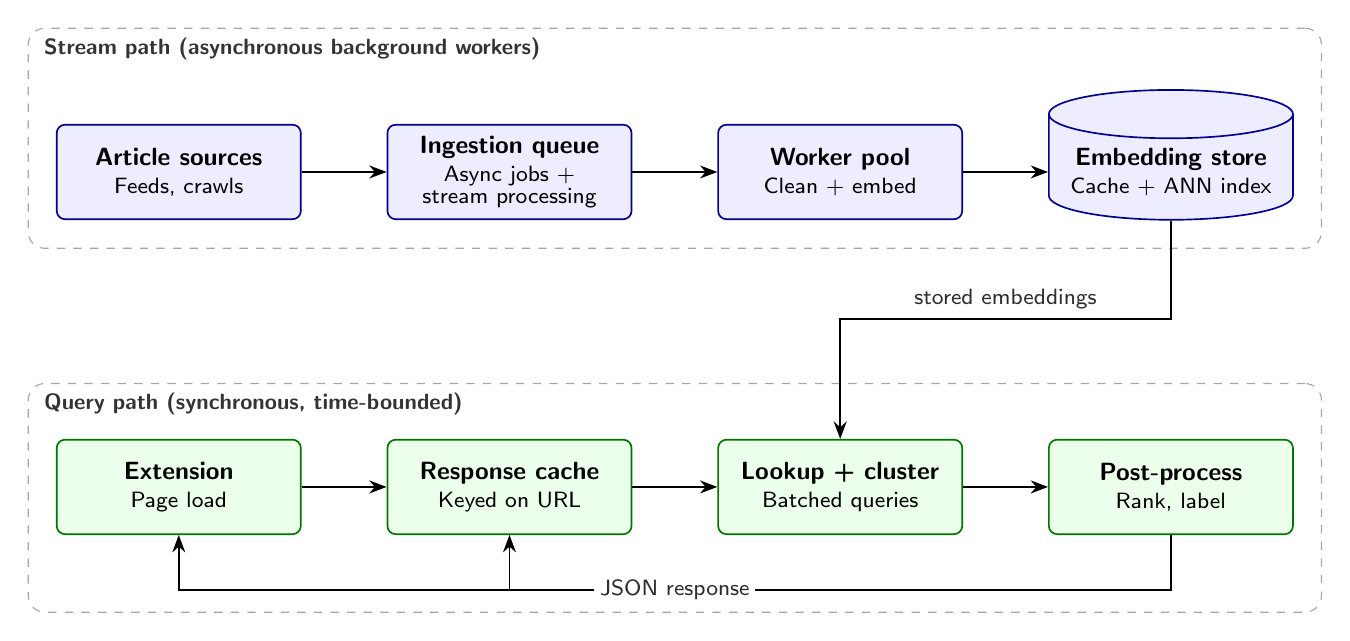
\begin{tikzpicture}[
  font=\sffamily\small,
  >={Stealth[length=2.2mm]},
  box/.style={draw, rounded corners=3pt, minimum width=3.1cm, minimum height=1.2cm, align=center, line width=0.6pt},
  sbox/.style={box, draw=blue!55!black, fill=blue!7},
  qbox/.style={box, draw=green!45!black, fill=green!8},
  grp/.style={draw=gray!70, dashed, rounded corners=6pt, inner sep=10pt},
  lab/.style={font=\sffamily\footnotesize\bfseries, text=gray!40!black, anchor=north west},
  sub/.style={font=\sffamily\footnotesize, text=gray!35!black}
]
% stream path
\node[sbox] (src) at (0,0)    {\textbf{Article sources}\\[-1pt]{\footnotesize Feeds, crawls}};
\node[sbox] (q)   at (4.2,0)  {\textbf{Ingestion queue}\\[-1pt]{\footnotesize Async jobs +}\\[-3pt]{\footnotesize stream processing}};
\node[sbox] (w)   at (8.4,0)  {\textbf{Worker pool}\\[-1pt]{\footnotesize Clean + embed}};
\node[cylinder, shape border rotate=90, aspect=0.22, draw=blue!55!black, fill=blue!7, line width=0.6pt,
      minimum width=3.1cm, minimum height=1.5cm, align=center] (st) at (12.6,0)
      {\textbf{Embedding store}\\[-1pt]{\footnotesize Cache + ANN index}};
\draw[->, line width=0.7pt] (src) -- (q);
\draw[->, line width=0.7pt] (q) -- (w);
\draw[->, line width=0.7pt] (w) -- (st);
\node[grp, fit=(src)(q)(w)(st), inner ysep=16pt, yshift=6pt] (g1) {};
\node[lab] at (g1.north west) {\;Stream path (asynchronous background workers)};

% query path
\node[qbox] (ext) at (0,-4)    {\textbf{Extension}\\[-1pt]{\footnotesize Page load}};
\node[qbox] (rc)  at (4.2,-4)  {\textbf{Response cache}\\[-1pt]{\footnotesize Keyed on URL}};
\node[qbox] (lk)  at (8.4,-4)  {\textbf{Lookup + cluster}\\[-1pt]{\footnotesize Batched queries}};
\node[qbox] (pp)  at (12.6,-4) {\textbf{Post-process}\\[-1pt]{\footnotesize Rank, label}};
\draw[->, line width=0.7pt] (ext) -- (rc);
\draw[->, line width=0.7pt] (rc) -- (lk);
\draw[->, line width=0.7pt] (lk) -- (pp);
\coordinate (ret) at ($(pp.south)+(0,-0.7)$);
\draw[->, line width=0.7pt] (pp.south) -- (ret) -| (ext.south);
\draw[->, line width=0.7pt] (rc.south |- ret) -- (rc.south);
\node[sub, fill=white, inner sep=2pt] at ($(ret)!0.5!(ret -| ext.south)$) {JSON response};
\node[grp, fit=(ext)(rc)(lk)(pp)(ret), inner ysep=14pt, yshift=6pt] (g2) {};
\node[lab] at (g2.north west) {\;Query path (synchronous, time-bounded)};

% store -> lookup
\draw[->, line width=0.9pt] (st.south) -- ++(0,-1.25) -| node[sub, pos=0.25, above] {stored embeddings} (lk.north);
\end{tikzpicture}}
\caption{System architecture. The stream path embeds every new article as it is published; the query path serves extension requests from the precomputed index.}
\end{figure}

\paragraph{Caching.}
\begin{itemize}
\item Per-article embeddings are cached and reused by any later user who views a page containing them.
\item Full API responses get a short-TTL cache keyed on page URL, so simultaneous viewers of the same popular page do not each trigger a separate lookup-and-cluster pass.
\end{itemize}

\paragraph{Batching.}
Queries are processed in batches: the headlines on one page go through the bi-encoder together in a single forward pass.

\paragraph{Async queues.}
Ingestion runs as a decoupled background worker pool, so a slow embedding job never blocks a page load. The query path stays synchronous but is bounded by a timeout, past which it falls back to the client side rather than leaving the user waiting.

\paragraph{Failure plan.}
On an index miss (a completely new article), the system falls back to an on-the-fly embedding in the browser client. If the backend is unreachable entirely, the extension renders the page unmodified rather than failing visibly.

\subsection{Latency/Accuracy Trade-offs}

\paragraph{Target SLOs.}
\begin{itemize}
\item p95 inference latency per page $\leq$ 50\,ms.
\item Test F1 $\geq$ 0.90 and PR-AUC $\geq$ 0.96 (the bi-encoder measured 0.906 and 0.966).
\end{itemize}

\paragraph{Shadow mode.}
When a newly fine-tuned bi-encoder is produced, whether to correct drift, to retrain on a label-noise-corrected pool or to expand outlet coverage, it first runs in shadow mode. Its predictions are logged internally and compared against the currently deployed model, and it is deployed only when it performs better.

\paragraph{Metrics to monitor.}
\begin{itemize}
\item Latency percentiles.
\item Score-distribution drift.
\item Backend error and timeout rate.
\item Index ``no match found'' rate.
\item Realized small-vs-major-outlet visibility ratio over time.
\end{itemize}

\end{document}
